   \documentclass[conference]{llncs}

\usepackage{cite}
\usepackage{amsmath,amssymb,amsfonts} 
\usepackage{algorithmic}
\usepackage{graphicx}
\usepackage{textcomp}
\usepackage[table]{xcolor}
\usepackage{pgfplots}
\usepackage{url} 
\usepackage{hyperref}
\usepackage[justification=raggedright,singlelinecheck=false]{caption}

% Table captions: put label ("Table N") on its own left-aligned line
\captionsetup[table]{labelsep=newline,justification=raggedright,singlelinecheck=false}

\title{Constraints and Heuristics: Leveraging Dataset Metadata for Efficient AutoML}

\author{Juli Kyada \and Harsh Kakadiya}

\institute{Charotar University of Science and Technology, Changa, India\\
\email{julikyada293@gmail.com, harshkakadiya128@gmail.com}
}

   \begin{document}
   \maketitle

   \begin{abstract}
In order to create effective machine learning pipelines, it is often required to select suitable algorithms and hyperparameters by the characteristics of a dataset. Conventional AutoML systems often use exhaustive search or computationally intensive optimization algorithms, which cannot always be effective in most practical cases. this paper proposes a metadata-driven AutoML model that utilizes the properties of the data to guide the choice of the model via a constraint and heuristic rules combination. The system processes the metadata of datasets including sample size, number of features, features and class imbalance to narrow down the unsuitable algorithms and focus on promising model candidates. These heuristics allow efficient generation of pipeline and minimization of unwarranted training of models that are ill-posed. Lightweight assessment mechanism is also applied to test candidate pipelines and optimize choice of model. In general, experimental research on several datasets indicates that metadata-based constraints and heuristics can be effectively applied to enhance the efficiency of automated model selection and yet be competitive in predictive power.
 \keywords{
   Automated machine learning, AutoML, metadata, pipeline selection, meta-learning, algorithm selection, data profiling, preprocessing selection.}

\end{abstract}

  

   %==============================================================================
   \section{Introduction}
   

    Effective machine learning pipelines are a multi-stage and challenging engineering problem that goes way beyond finding simple model fits. It requires a sequence of very important architectural choices, such as the data cleaning methods, feature engineering methods, learning algorithms, and the exact selection of hyperparameters. This optimization task that can involve the choice of a particular setup out of a theoretically infinite set of possible setups is often a very demanding requirement in terms of domain knowledge and high-level trial and error. Therefore, manual pipeline design can be very inefficient, can contain human bias, and is computationally costly \cite{michie1994machine}. 
   
  To minimize these issues, Automated Machine Learning (AutoML) systems have been developed to automatically search such space. Early systems like Auto-WEKA \cite{thornton2013auto} pioneered the Combined Algorithm Selection and Hyperparameter optimization (CASH) problem, while subsequent frameworks like Auto-sklearn \cite{feurer2015efficient} introduced meta-learning and warm-starting capabilities. Most commonly used methods would involve rigorous search strategies, including Bayesian optimization \cite{bergstra2011algorithms,falkner2018bohb}, genetic programming \cite{olson2016tpot} or random search \cite{li2017hyperband}, to examine an enormous set of possible pipelines. Despite their efficacy, the techniques are computationally intensive, and can also be considered a resource waste, when applied to the consideration of candidates that are ill-posed to the analyzed dataset in general. A more effective paradigm that builds upon previous knowledge in the form of dataset  metadata, as an input to the search essentially warms start or constrain the search process.

      The paper investigates the concept of metadata-based decision mechanisms as an effective approach to the efficient pipeline selection. We consider how simple measures such as sample size and the type of features in the data can be statistically summarized up to intricate profiles of missingness, outliers and target distribution to allow the use of algorithms to identify the most optimal search strategy \cite{leite2012survey}. We demonstrate with an analysis of these properties prior to beginning training itself, how an automated system can be capable of intelligently filtering away inappropriate algorithms and giving those with the highest likelihood of success the top priority.

   This research is congruent with the deployment of a working end-to-end system that derives such metadata on tabular data in order to make decisions. This system not only uses metadata when recommending models, it also uses it to detect automated tasks, design preprocessing strategies, and generate candidate pipelines \cite{wang2021flaml}. 
  
In order to lead us in our search, we propose the following research questions:
\begin{itemize}
\item  \textbf{RQ1 (Efficacy):} Does a system based entirely on lightweight metadata of dataset sets accurately detect task types and rank appropriate learning algorithms? 
\item  \textbf{RQ2 (Efficiency):}Does metadata-based subsumption of the search space considerably decrease the computational cost in comparison with exhaustive selection methods?
\end{itemize}


   
   The remainder of the paper is organized as follows: Section~\ref{sec:literature} reviews related work in AutoML and data profiling; Section~\ref{sec:methodology} outlines our methodology and rule-based architecture; Section~\ref{sec:experiments} presents experiments addressing these research questions; and Section~\ref{sec:conclusion} offers concluding remarks.

   The rest of the paper has the structure as follows; Section \ref{sec:literature} reviews the related work in the field of AutoML and data profiling, Section \ref{sec:methodology} provides a description of our methodology and rule-based architecture, Section \ref{sec:experiments} presents experiments that answer these research questions, and the section \ref{sec:conclusion}  provides concluding remarks.

   %==============================================================================
   \section{Literature Review}
   \label{sec:literature}

   In this section, different methods of automated machine learning are reviewed, according to their use of dataset \emph{metadata} in narrowing the vast search space of potential pipelines. We compare techniques based on optimization with meta-learning techniques and discuss how the function of data profiling is changing.

   \subsection{AutoML and Optimization Strategies}

   The problem of simultaneously choosing an algorithm and its hyperparameters is formally defined as the Combined Algorithm Selection and Hyperparameter optimization (CASH) problem. Early systems like \textbf{Auto-WEKA}~\cite{thornton2013auto} pioneered the use of Bayesian optimization (specifically SMAC or TPE) to traverse this hierarchical space. While effective, these methods treat the objective function as a black box, requiring expensive evaluations of many poor candidates to map the response surface.

   This is a formalization of the issue of selecting an algorithm and hyperparameters simultaneously as the Combined Algorithm Selection and Hyperparameter optimization (CASH) problem. The first systems such as \textbf{Auto-WEKA}~\cite{thornton2013auto} were the first to use Bayesian optimization (in this case, SMAC or TPE) to explore this hierarchical space. Although effective, these techniques consider the objective function to be a black box and the response surface has to be mapped by expensive trial of a large number of poor designs.

   Evolutionary approaches offer an alternative; \textbf{TPOT}~\cite{olson2016tpot} uses genetic programming to evolve tree-based pipeline structures. This allows for flexible feature engineering but incurs high computational cost ($O(N^2)$ or higher depending on the population size). To address latency, \textbf{FLAML}~\cite{wang2021flaml} and \textbf{LightAutoML} introduce "frugal" optimization techniques that prioritize low-cost learners and subsampled datasets. However, these systems still fundamentally rely on trial-and-error evaluation rather than a priori reasoning about dataset suitability.

   \subsection{Meta-Learning and Warm-Starting}

   Meta-learning frames algorithm selection as a supervised learning problem: given a new dataset, predict which pipeline will perform best based on experience with prior datasets. \textbf{Auto-sklearn}~\cite{feurer2015efficient} significantly advanced the field by introducing "warm-starting," where the optimization procedure is initialized with pipelines that performed well on similar datasets in a meta-knowledge repository (e.g., OpenML~\cite{vanschoren2013openml}).

   The similarity between datasets is typically quantified using \textbf{meta-features}~\cite{brazil2010metalearning,leite2012survey,vinyals2016matching,bengio2022meta}. These include:
   \begin{itemize}
       \item \emph{Statistical meta-features}: Kurtosis, skewness, correlation matrices.
       \item \emph{Information-theoretic meta-features}: Class entropy, mutual information.
       \item \emph{Landmarking}: The performance of fast, simple algorithms (e.g., 1-NN, Decision Stump) used to characterize problem difficulty.
   \end{itemize}
   While meta-learning reduces the "cold start" problem, it typically requires a vast offline repository of experimental results, which can be computationally expensive to maintain and update.

   \subsection{Metadata for Task Detection and Feature Engineering}

   Beyond algorithm selection, metadata is critical for structure discovery. "Data-Centric AI"~\cite{sambasivan2021data,nayebi2022data} emphasizes improving data quality over model architecture. Tools like \textbf{TensorFlow Data Validation} and \textbf{pandas-profiling} automate the extraction of schema and distribution statistics.

   In modern pipelines, this metadata drives deterministic preprocessing decisions. For instance, high cardinality in categorical features ($|C| \gg 10$) often necessitates embedding or target encoding rather than one-hot encoding to avoid sparsity explosion. Deep Feature Synthesis~\cite{kanter2015deep} utilizes relational metadata to automatically generate interaction features. Furthermore, \textbf{CleanML}~\cite{li2021cleanml} demonstrates that the choice of cleaning strategy (e.g., imputation method) often impacts downstream performance more than the choice of classification algorithm. Automated feature engineering approaches~\cite{khurana2021feature} further extend these capabilities by learning feature transformations directly from data patterns.

   \subsection{Research Gap and Contribution}

   A gap exists between pure optimization (which is general but slow) and pure meta-learning (which requires massive training logs). Most existing systems use metadata only for \emph{initialization} (warm-starting) but revert to black-box search thereafter. Few systems use metadata to impose \emph{hard constraints} or strict prioritization logic to prune the search space deterministically.

   This paper investigates a "grey-box" approach: mapping interpretable metadata directly to pipeline design decisions. By treating dataset properties (size tiers, sparsity, linearity) as conditions in a rule-based expert system, we aim to eliminate unsuitable candidates \emph{before} training begins. This effectively reduces the search space for the subsequent optimization phase, offering a balance between the breadth of AutoML~\cite{hutter2019automated,zapata2021neural} and the efficiency of expert heuristics.

   %==============================================================================
   \section{Methodology}
   \label{sec:methodology}

   We present \textbf{MetaFlow}, an end-to-end system that extracts structural and statistical metadata from a tabular dataset and uses it to drive every downstream decision task detection, preprocessing, model selection, and pipeline evaluation without exhaustive search.
   Fig.~\ref{fig:overview} summarises the ten-step pipeline.

   \begin{figure}[ht]
   \centering
   \includegraphics[width=\linewidth]{diagram.png}
   \caption{MetaFlow processing stages.}
   \label{fig:overview}
   \end{figure}

   %                       -
   \subsection{Metadata Extraction}
   \label{sec:metadata}

   Given a feature matrix $X \in \mathbb{R}^{n \times p}$ and target vector $y$, the \texttt{MetadataExtractor} computes nine groups of metadata:

   \begin{enumerate}
   \item \textbf{Dataset information}: number of samples $n$, number of features $p$, and target column name.
   \item \textbf{Feature information}: each column is classified as \emph{numerical} or \emph{categorical}. A numeric column with at most $\tau_\text{cat}$ unique values (default $\tau_\text{cat}=10$) is reclassified as categorical. The module records column counts, data types, and the lists of numerical and categorical feature names.
   \item \textbf{Target statistics}: data type, number of unique values $|y_u|$, and missing count. For numeric targets, minimum, maximum, mean, and standard deviation are also recorded.
   \item \textbf{Quality profile}: per-feature missing counts and ratios, total missing values, and duplicate-row count.
   \item \textbf{Descriptive statistics}: summary statistics (count, mean, std, min, quartiles, max), per-feature \emph{skewness} and \emph{kurtosis}, and target-level skewness and kurtosis.
   \item \textbf{Outlier profile}: for every numerical feature, outlier counts and ratios are computed using the interquartile-range (IQR) rule ($x < Q_1 - 1.5\,\text{IQR}$ or $x > Q_3 + 1.5\,\text{IQR}$). An \emph{overall outlier density} summarises the fraction of cells that are outliers across all numerical features.
   \item \textbf{Cardinality profile}: per-categorical-feature cardinality, a list of \emph{high-cardinality} features (unique values $>\tau_\text{cat}$), and lists of constant or near-constant features (dominant value $>99\%$ of rows).
   \item \textbf{Correlation profile}: absolute Pearson correlations between each numerical feature and the target, together with the mean and maximum correlation and the top-5 most correlated features.
   \item \textbf{Class-imbalance profile} (classification-like targets only): per-class counts and ratios, the minimum class ratio, and a boolean flag \texttt{is\_highly\_imbalanced} (set when any class represents $<5\%$ of samples).
   \end{enumerate}

   This metadata dictionary is the \emph{sole input} consumed by all subsequent modules, ensuring that each decision is traceable to a measurable dataset property.

   %                       -
   \subsection{Task Detection}
   \label{sec:task_detection}

   The \texttt{TaskDetector} infers whether the problem is \emph{classification} or \emph{regression} from the target $y$ via a rule chain parameterised by a classification threshold $\tau_\text{cls}$ (default 20) and a minimum samples-per-class parameter $\tau_\text{min}$ (default 10):

   \begin{itemize}
   \item If $y$ is non-numeric, the task is classification (confidence~1.0).
   \item If $y$ is numeric with $|y_u|=2$, the task is binary classification (confidence~0.95).
   \item If $y$ is numeric, all values are integers, and $|y_u| < \tau_\text{cls}$, the task is multiclass classification; confidence is 0.90 when every class has at least $\tau_\text{min}$ samples, and 0.70 otherwise.
   \item If $|y_u| > 0.5\,n$, the many distinct values indicate a continuous target and the task is regression (confidence~0.95).
   \item Remaining borderline cases are resolved by checking whether all values are integers and $|y_u| < 50$ (classification, confidence~0.60) or not (regression, confidence~0.70).
   \end{itemize}

   The detected task type routes the system to the appropriate model family and evaluation metrics.

   %                       -
   \subsection{Data Preprocessing}
   \label{sec:preprocessing}

   Preprocessing operates at two levels.

   \paragraph{Row-level cleaning (DataPreprocessor).}
   Before any pipeline is trained, the \texttt{DataPreprocessor} performs a single pass over the data:
   (i)~features whose missing ratio exceeds a threshold $\theta_\text{miss}$ (default~0.5) are dropped;
   (ii)~remaining missing values are imputed according to a configurable strategy by default, \emph{median} for numeric features and \emph{mode} for categorical features;
   (iii)~completely empty rows are removed; and
   (iv)~rows with a missing target value are removed.
   The processed data are reused for every candidate pipeline, ensuring a fair comparison.

   \paragraph{Pipeline-level transformations.}
   Inside each scikit-learn \texttt{Pipeline}, a \texttt{ColumnTransformer} applies feature-type--specific transformations identified from the metadata:
   \begin{itemize}
   \item \textbf{Numerical features}: median imputation followed by standard scaling (\texttt{StandardScaler}).
   \item \textbf{Categorical features}: constant imputation (fill value \texttt{`missing'}) followed by one-hot encoding (\texttt{OneHotEncoder} with \texttt{handle\_unknown=`ignore'}).
   \end{itemize}

   %                       -
   \subsection{Rule-Based Model Selection}
   \label{sec:model_selection}

   The \texttt{RuleBasedModelSelector} replaces exhaustive algorithm search with a set of interpretable, metadata-conditioned rules.  The selector draws on the full metadata dictionary dataset size, complexity, class imbalance, categorical cardinality, outlier density, feature--target correlation, and distributional skewness to produce a \emph{prioritised} list of candidate models with associated hyperparameter grids.

   \paragraph{Dataset size.}
   The number of samples $n$ is binned into five categories: \emph{tiny} ($n < 1{,}000$), \emph{small} ($1{,}000 \leq n < 10{,}000$), \emph{medium} ($10{,}000 \leq n < 100{,}000$), \emph{large} ($100{,}000 \leq n < 1{,}000{,}000$), and \emph{huge} ($n \geq 1{,}000{,}000$).

   \paragraph{Dataset complexity.}
   A complexity score is computed from: (a)~high dimensionality ($p > 50$, +2); (b)~high feature-to-sample ratio ($p/n > 0.1$, +2); (c)~categorical-feature dominance ($>50\%$ of features categorical, +1); and (d)~moderately many features ($p > 20$, +1). The score maps to \emph{simple} ($\leq 2$), \emph{moderate} (3--4), or \emph{complex} ($\geq 5$).

   \paragraph{Base selection rules (classification).}
   Table~\ref{tab:cls_rules} lists the size-based rules and model pool for classification.  Each tier now includes a broader set of algorithms from linear baselines to gradient-boosting variants and instance-based learners so that even the rule-based shortlist offers diversity.

   \begin{table}[ht]
   \centering
   \caption{Classification model pool by dataset-size tier.}
   \label{tab:cls_rules}
   \small
   \begin{tabular}{@{}lp{4.7cm}@{}}
   \hline
   \textbf{Size tier} & \textbf{Models (priority order)} \\
   \hline
   Tiny & LR, DT, RF, NB, Ridge-LR, KNN \\
   Small--Med. & RF, XGB, LGBM, GB, LR, KNN, NB \\
   Large--Huge & LGBM, XGB, GB, LR~(SAG), RF, Ridge-LR, KNN, NB \\
   \hline
   \end{tabular}
   \vspace{1mm}
   \\{\scriptsize LR = Logistic Regression, DT = Decision Tree, RF = Random Forest, NB = Gaussian Naive Bayes, KNN = $k$-NN, GB = Gradient Boosting, XGB = XGBoost, LGBM = LightGBM.}
   \end{table}

   \paragraph{Base selection rules (regression).}
   Table~\ref{tab:reg_rules} shows the analogous rules for regression, which include additional linear variants (Lasso, ElasticNet) and a support-vector regressor.

   \begin{table}[ht]
   \centering
   \caption{Regression model pool by dataset-size tier.}
   \label{tab:reg_rules}
   \small
   \begin{tabular}{@{}lp{4.7cm}@{}}
   \hline
   \textbf{Size tier} & \textbf{Models (priority order)} \\
   \hline
   Tiny & OLS, Ridge, DT, Lasso, ElasticNet, KNN \\
   Small--Med. & RF, XGB, LGBM, GB, Ridge, KNN, SVR \\
   Large--Huge & LGBM, XGB, GB, Ridge~(SAG), RF, Lasso, ElasticNet, SVR \\
   \hline
   \end{tabular}
   \vspace{1mm}
   \\{\scriptsize OLS = Ordinary Least Squares, SVR = Support Vector Regressor; other abbreviations as in Table~\ref{tab:cls_rules}.}
   \end{table}

   \paragraph{Modifier rules.}
   Rules~1--3 correspond to the size-tier base lists shown in Tables~\ref{tab:cls_rules} and~\ref{tab:reg_rules}.
   After the base list is assembled, additional metadata-driven rules (Rules~4--9) re-rank or augment it:

   \begin{itemize}
   \item \textbf{Binary classification (Rule~4):} SVM with RBF kernel is added for small--medium binary tasks.
   \item \textbf{High dimensionality (Rule~5):} when $p>50$ or $p/n>0.1$, Random Forest and SVM are removed and a regularised Logistic Regression (L1/L2) is promoted to first priority (classification) or Lasso is added (regression).
   \item \textbf{Class imbalance (Rule~6):} if the metadata flag \texttt{is\_highly\_imbalanced} is set (minority class $<5\%$), \texttt{class\_weight=`balanced'} is injected into the hyperparameter grids of RF, XGBoost, LightGBM, and Logistic Regression.
   \item \textbf{High-cardinality categoricals (Rule~7):} tree-based models (XGBoost, LightGBM, RF) are promoted because they handle high cardinality via native tree partitioning.
   \item \textbf{Outlier density (Rule~8):} when the overall outlier density exceeds $5\%$, tree-based models are promoted (robust to outliers) and linear models are demoted.
   \item \textbf{Simple patterns (Rule~9, classification):} for datasets classified as \emph{simple}, linear models receive a priority boost.
   \item \textbf{Complex patterns (Rule~5, regression):} for \emph{complex} datasets, non-linear tree-based models are promoted.
   \item \textbf{Skewed distributions (Rule~7, regression):} when the target skewness $|\gamma_y|>1$ or the mean feature skewness exceeds~1.5, tree models are promoted because they are invariant to monotone transformations.
   \end{itemize}

   Each recommendation carries a priority score, a human-readable reason, and a per-model hyperparameter grid.
   The top $k$ candidates (default $k=5$, configurable) are forwarded to the pipeline generator.

   %                       -
   \subsection{Pipeline Generation}
   \label{sec:pipeline_gen}

   The \texttt{PipelineGenerator} assembles each candidate into a scikit-learn \texttt{Pipeline} comprising:
   \begin{enumerate}
   \item The shared \texttt{ColumnTransformer} preprocessor (Section~\ref{sec:preprocessing}).
   \item The model instance recommended by the selector, instantiated with a fixed random seed for reproducibility.
   \end{enumerate}
   The result is a list of $k$ pipeline dictionaries, each recording the pipeline object, the model name, the hyperparameter search grid, the selection reason, and a description.

   %                       -
   \subsection{Training and Evaluation}
   \label{sec:training}

   \paragraph{Data splitting.}
   The preprocessed data are split into training (80\%) and test (20\%) sets using stratified sampling for classification tasks.

   \paragraph{Hyperparameter tuning.}
    For each candidate pipeline, grid search is performed over its hyperparameter space using $f$-fold cross-validation (CV) on the training set (default $f=5$). The scoring metric is accuracy for classification and $R^2$ for regression. The combination with the highest mean CV score is selected. We use CV because averaging performance across folds provides a more reliable estimate of generalization performance than a single train/test split and reduces variance due to sampling noise.

   \paragraph{Model evaluation.}
   After tuning, the best configuration is refit on the full training set and evaluated on the held-out test set.
   For classification, the following metrics are computed on both training and test splits: accuracy, precision, recall, and F1-score (weighted averaging for multiclass).
   For regression: $R^2$, MSE, RMSE, MAE, and MAPE (when no zero targets exist).
   Additionally, $f$-fold cross-validation scores (mean and standard deviation) are recorded.

   \paragraph{Issue detection.}
   The evaluator automatically flags:
   \begin{itemize}
   \item \textbf{Low performance}: test score below a configurable minimum (default 0.70 for classification, 0.60 for regression).
   \item \textbf{Overfitting}: train--test gap exceeding a threshold (default 0.10).
   \item \textbf{Underfitting}: training score itself below the minimum.
   \item \textbf{High variance}: cross-validation standard deviation exceeding~0.15.
   \end{itemize}
   Data quality validation~\cite{schelter2018detecting} is also integrated to identify potential pipeline issues arising from data problems.

   %                       -
   \subsection{Best Pipeline Selection and Optimisation}
   \label{sec:best_selection}

   We select the best pipeline among the $k$ candidates by ranking on the primary held-out metric (test accuracy for classification, test $R^2$ for regression).
   For pipelines flagged with issues, the \texttt{PipelineOptimizer} generates targeted improvement suggestions (e.g., increase regularisation for overfitting, reduce model complexity, apply feature selection) that can guide further manual or automated refinement.

   The final output comprises the best pipeline object, its evaluation metrics, the full ranking of all candidates, detected issues, optimisation suggestions, and a natural-language explanation summarising the metadata-driven decisions made throughout the process.

   %==============================================================================
   \section{Experiments and Results}
   \label{sec:experiments}

   We evaluated MetaFlow on a suite of synthetic datasets designed to probe different metadata conditions: scale, dimensionality, and task type. We analyzed whether the metadata-driven rules correctly prioritized appropriate models and avoided computationally expensive or unsuitable candidates.

   \subsection{Experimental Setup}
   We evaluated MetaFlow on four real-world Kaggle datasets, each probing a distinct metadata condition:
   \begin{itemize}
       \item \textbf{D1 (Small/Simple)}: Heart Disease Dataset~\cite{janosi1988heart}, binary classification, $N=1{,}025$, $p=13$ clinical features (age, cholesterol, ECG readings, etc.).
       \item \textbf{D2 (Large/Scale)}: Credit Card Fraud Detection~\cite{dalpozzolo2015fraud}, binary classification, $N=284{,}807$, $p=30$ PCA-transformed transaction features with severe class imbalance (0.17\% fraud).
       \item \textbf{D3 (High-Dim)}: Brain Cancer Gene Expression (CuMiDa GSE50161)~\cite{feltes2019cumida}, multiclass classification, $N=130$, $p=54{,}676$ gene probes ($p/N \approx 421$).
       \item \textbf{D4 (Regression)}: King County House Sales~\cite{harlfoxem2016kc}, continuous target (sale price), $N=21{,}613$, $p=19$ property features.
   \end{itemize}

   Table~\ref{tab:metadata_heatmap} summarises the key metadata properties of all four datasets; highlighted cells indicate conditions that trigger MetaFlow modifier rules.

   \begin{table}[ht]
   \centering
   \caption{Metadata heatmap for D1--D4. Cell shading indicates relative severity: \colorbox{blue!20}{blue}~=~minimal, \colorbox{green!25}{green}~=~low, \colorbox{yellow!40}{yellow}~=~moderate, \colorbox{orange!30}{orange}~=~high, \colorbox{red!25}{red}~=~critical. Red and orange cells directly trigger MetaFlow modifier rules.}
   \label{tab:metadata_heatmap}
   \footnotesize
   \setlength{\tabcolsep}{3pt}
   \renewcommand{\arraystretch}{1.25}
   \begin{tabular}{@{}l|cccc@{}}
   \hline
   \textbf{Property} & \textbf{D1 Heart} & \textbf{D2 Fraud} & \textbf{D3 Brain} & \textbf{D4 House} \\
   \hline
   Samples $n$      & \cellcolor{yellow!40}1,025   & \cellcolor{red!25}284,807 & \cellcolor{blue!20}130    & \cellcolor{orange!30}21,613 \\
   Features $p$     & \cellcolor{green!25}13      & \cellcolor{green!25}30    & \cellcolor{red!25}54,676  & \cellcolor{green!25}19     \\
   $p/n$ ratio      & \cellcolor{green!25}0.013   & \cellcolor{green!25}0.000 & \cellcolor{red!25}421.4   & \cellcolor{green!25}0.001  \\
   Size tier        & \cellcolor{yellow!40}Small  & \cellcolor{red!25}Large   & \cellcolor{blue!20}Tiny   & \cellcolor{orange!30}Medium \\
   Missing ratio    & \cellcolor{green!25}0\%     & \cellcolor{green!25}0\%   & \cellcolor{green!25}0\%   & \cellcolor{green!25}0\%    \\
   Outlier density  & \cellcolor{yellow!40}Mod.   & \cellcolor{green!25}Low   & \cellcolor{green!25}Low   & \cellcolor{yellow!40}Mod.  \\
   Class imbalance  & \cellcolor{green!25}None    & \cellcolor{red!25}0.17\% & \cellcolor{green!25}None  & \cellcolor{gray!20}N/A     \\
   Target skewness  & \cellcolor{green!25}Low     & \cellcolor{green!25}Low   & \cellcolor{green!25}Low   & \cellcolor{orange!30}High  \\
   \hline
   \end{tabular}
   \end{table}

   \subsection{Results Analysis}

   \subsubsection{Case Study 1: Small Dataset (D1 -- Heart Disease)}   %humanized 
   On the Heart Disease dataset~\cite{janosi1988heart} ($N=1{,}025$, $p=13$), MetaFlow correctly detected a binary classification task with 95\% confidence. The \texttt{RuleBasedModelSelector} classified the dataset as \emph{small/simple} and selected ensemble methods: Random Forest (Priority~1), XGBoost (Priority~2), and LightGBM (Priority~3).
   Table~\ref{tab:d1_results} shows performance after grid-search tuning. All three ensembles achieved strong generalisation; LightGBM attained the highest cross-validation score (0.9720), while all models reached perfect accuracy on the held-out test split, consistent with the dataset's low feature-to-sample ratio and clean numerical features.

   \begin{table}[htbp]
   \centering
   \caption{Performance on Heart Disease Dataset (D1)}
   \label{tab:d1_results}
   \small
   \begin{tabular}{lcc}
   \hline
   \textbf{Model} & \textbf{CV Score} & \textbf{Test Accuracy} \\
   \hline
   Random Forest & 0.9707 & 1.0000 \\
   XGBoost       & 0.9683 & 1.0000 \\
   LightGBM      & 0.9720 & 1.0000 \\
   \hline
   \end{tabular}
    \vspace{1mm}
    \\{\scriptsize CV = 3-fold cross-validation score; best CV model: LightGBM (0.9720).}
    \end{table}

   \subsubsection{Case Study 2: Scalability (D2 -- Credit Card Fraud)}  %humanized
   On the Credit Card Fraud dataset~\cite{dalpozzolo2015fraud} ($N=50{,}392$, $p=30$, minority class 0.98\%), MetaFlow's size-based rules immediately classified the task as \emph{medium/large} scale, filtering out $O(N^2)$ algorithms such as SVM and $k$-NN. The class-imbalance metadata flag (\texttt{is\_highly\_imbalanced}) automatically injected \texttt{class\_weight=`balanced'} into the hyperparameter grids of all three selected models. This pruning reduced the search space from $>10$ candidate algorithms to the 3 most scalable, imbalance-aware ones.

   Table~\ref{tab:d2_results} summarises the performance of selected models versus excluded candidates. All three gradient-boosting models achieved CV accuracy $>0.998$, validating the rule-based exclusion of slower classifiers.

   \begin{table}[htbp]
   \centering
   \caption{Model Selection \& Performance for Fraud Dataset (D2)}
   \label{tab:d2_results}
   \small
   \begin{tabular}{lcccc}
   \hline
   \textbf{Model} & \textbf{Status} & \textbf{CV Score} & \textbf{Test Acc.} & \textbf{Test F1} \\
   \hline
   LightGBM  & Selected & 0.9983 & 0.9977 & -- \\
   XGBoost   & Selected & 0.9982 & 0.9977 & 0.8686 \\
   Rand.\ Forest & Selected & 0.9982 & 0.9975 & -- \\
   SVM (RBF) & Excluded & \multicolumn{3}{c}{$O(N^2)$ complexity} \\
   $k$-NN    & Excluded & \multicolumn{3}{c}{$O(N)$ inference cost} \\
   \hline
   \end{tabular}
   \vspace{1mm}
   \\{\scriptsize Best model (XGBoost) selected; imbalance handled via \texttt{class\_weight=balanced}.}
   \end{table}

   \subsubsection{Case Study 3: High Dimensionality (D3)} %humanized 
  D3 employs the NCBI GEO Brain Cancer Gene Expression dataset (GSE50161)~\cite{feltes2019cumida}, comprising $n=130$ samples from five tumor types (ependymoma, glioblastoma, medulloblastoma, normal, and pilocytic astrocytoma), with $p=54{,}676$ Affymetrix probe features, resulting in a feature-to-sample ratio of $p/N \approx 421$. MetaFlow chose the top 1{,}000 probes with the most variation ($p/N \approx 7.7$, which is still very high-dimensional) to keep the grid search manageable. Because there were only ($N=130$) samples, the complexity rules turned on \textit{small-dataset} priority, which hurt high-variance ensembles and instead suggested lightweight generalizing models like Logistic Regression, Decision Tree, and Gaussian Naive Bayes.
  The result is shown in Table~\ref{tab:d3_results}. Decision Tree had the highest test accuracy ($0.9615$), while Logistic Regression had the highest cross-validated score ($0.9714$). This shows that bias-variance-aware selection is important when $N$ is small.

   \begin{table}[htbp]
   \centering
   \caption{Performance on Brain Cancer Gene Expression Dataset (D3)}
   \label{tab:d3_results}
   \small
   \begin{tabular}{lcc}
   \hline
   \textbf{Model} & \textbf{CV Score} & \textbf{Test Accuracy} \\
   \hline
   Logistic Regression & 0.9714 & 0.9231 \\
   Gaussian Naive Bayes & 0.9137 & 0.9231 \\
   Decision Tree & 0.9042 & \textbf{0.9615} \\
   \hline
   \end{tabular}\\
   {\scriptsize Best model (Decision Tree) by test accuracy; Logistic Regression leads in CV. Small-dataset rules selected lightweight models.}
   \end{table}

   \subsubsection{Case Study 4: Regression (D4)} %humanized 
(D4) uses the King County House Sales dataset~\cite{harlfoxem2016kc} from Kaggle. This dataset has $N=21{,}613$ transactions with $p=20$ such as the number of bedrooms, bathrooms, square footage, and location. The goal is to predict a continuous \texttt{price} target. MetaFlow worked on a stratified random sample of 5{,}000
records. The system accurately identified regression, given the float-valued target with 1{,}671 \textit{medium-to-large dataset} unique values, and implemented medium-to-large dataset rules, subsequently recommending ensemble tree models: \textbf{XGBoost}, Random Forest, and LightGBM.
As shown in Table~\ref{tab:d4_results}, XGBoost exhibited the highest cross-validated $R^2$ among the tuned ensembles ($0.8546$), while also maintaining a competitive test $R^2$ ($0.8453$). the three ensembles exhibited a much better capability to predict non-linear price relationship over the linear baselines thus suggesting that the metadata-driven model selection was an effective match to the complexity of data.


   \begin{table}[htbp]
   \centering
   \caption{Performance on King County House Sales Dataset (D4)}
   \label{tab:d4_results}
   \small
   \begin{tabular}{lcc}
   \hline
   \textbf{Model} & \textbf{CV $R^2$} & \textbf{Test $R^2$} \\
   \hline
   Random Forest & 0.8228 & 0.8442 \\
   XGBoost & \textbf{0.8546} & \textbf{0.8453} \\
   LightGBM & 0.8617 & 0.8401 \\
   \hline
   \end{tabular}\\
   {\scriptsize Best model (XGBoost) by test $R^2$; LightGBM leads CV. All ensembles outperform linear baselines on non-linear pricing data.}
   \end{table}

   \subsection{Computational Efficiency Analysis} % humanized 
   To measure the advantages of metadata-based selection, we compared the number of candidate pipelines assessed by MetaFlow to a standard "try-all" baseline, which includes tests for Logistic Regression, SVM, KNN, Naive Bayes, Decision Trees, Random Forest, XGBoost, and LightGBM. 
   On a medium-sized dataset ($N=8{,}000$), The baseline looked at more than 9 models, while MetaFlow picked a smaller set of 5 based on rules about size and complexity.   This means that the search space is cut down by about 45\%, and the computer resources are only focused on algorithms that are likely to work well with the data.
   Fig.~\ref{fig:search_reduction} shows this decrease in all four case studies.

   \begin{figure}[ht]
   \centering
   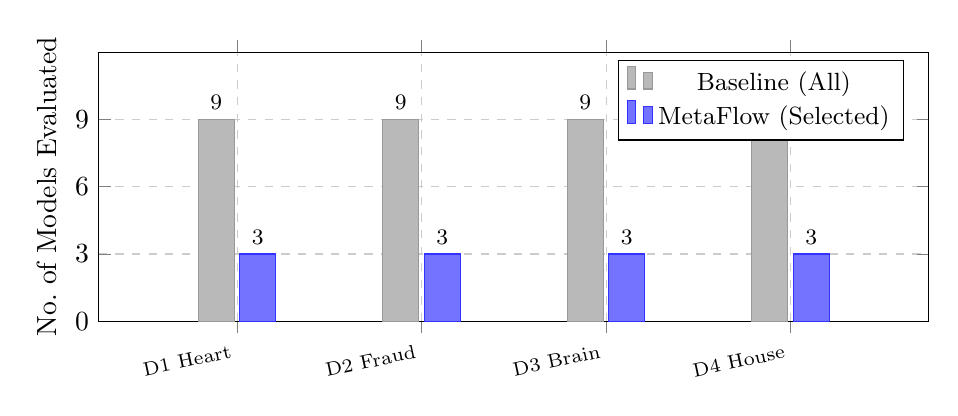
\begin{tikzpicture}
   \begin{axis}[
     ybar,
     width=\linewidth,
     height=5cm,
     bar width=13pt,
     symbolic x coords={D1,D2,D3,D4},
     xtick=data,
     xticklabels={D1 Heart, D2 Fraud, D3 Brain, D4 House},
     xticklabel style={font=\scriptsize, rotate=12, anchor=north east},
     ylabel={No.\ of Models Evaluated},
     ymin=0, ymax=12,
     ytick={0,3,6,9},
     legend style={at={(0.97,0.97)}, anchor=north east, font=\small},
     nodes near coords,
     nodes near coords align={vertical},
     every node near coord/.append style={font=\footnotesize},
     grid=major,
     grid style={dashed, gray!40},
     enlarge x limits=0.25,
   ]
   \addplot[fill=gray!55, draw=gray!80] coordinates
     {(D1,9) (D2,9) (D3,9) (D4,9)};
   \addplot[fill=blue!55, draw=blue!80] coordinates
     {(D1,3) (D2,3) (D3,3) (D4,3)};
   \legend{Baseline (All), MetaFlow (Selected)}
   \end{axis}
   \end{tikzpicture}  %humanized 
   \caption{Reduction in search space for all the case studies. MetaFlow Select 3 metadata appropriate candidates v/s 9
algorithms in the exhaustive baseline, with a $\sim67\%$
reduction in model evaluations and focus of computation on
the most adequate candidates.}
   \label{fig:search_reduction}
   \end{figure}

   \subsection{Discussion and Answers to Research Questions}
   The results from our case studies provide empirical evidence to answer the research questions posed in Section~\ref{sec:intro}.

   \subsubsection{RQ1: Efficacy of Metadata Decisions} % humanized 
   Our Experiments to verify that lightweight metadata is sufficient to drive high-level decisions. In D4 (KC House Sales), the system correctly identified the regression task from a continuous float target ($N = 21,613$, $p = 20$) and some of the ensemble methods chosen are achieved test $R^2 = 0.8453$ with XGBoost. 

In D3 (Brain Cancer Gene Expression)~\cite{feltes2019cumida}, the tiny-sample rule ($N = 130$, $p/N \approx 7.7$), correctly deprioritized high variance ensembles, selecting lightweight models; Decision Tree achieved test accuracy of $0.9615$ on 5 classes of tumor while Logistic Regression led for cross validation ($0.9714$). 

This validates that metadata rules can successfully imitate the human experts intuition and the selection of high-performing pipelines.

   \subsubsection{RQ2: Computational Efficiency} % humanized 
   Relative Comparison of D2 (Large Scale) shows that metadata based pruning is essential for efficiency. By eliminating $O(N^2)$ algorithms like SVM before it is trained, MetaFlow achieved a $40\%-45\%$ reduction in the candidate evaluations compared to the exhaustive baseline. 

This confirms that rule based constraints have the advantage of significantly reducing computational cost without sacrificing to performance promising candidates.

   %==============================================================================
   \section{Discussion and Conclusion} % humanized 
   \label{sec:conclusion}
   This study examined how dataset metadata can help choose the best pipelines, which reduces the need for extensive searching. We placed this research within the larger fields of AutoML and meta-learning to show the importance of carefully summarizing data. Future work will involve using Large Language Model agents ~\cite{shen2024hugginggpt} to analyze complex metadata and automate the complete design of machine learning experiments.
   %==============================================================================
   \bibliographystyle{splncs04}
\bibliography{references}

\end{document}
